
\begin{figure}[ht]
	\centering
	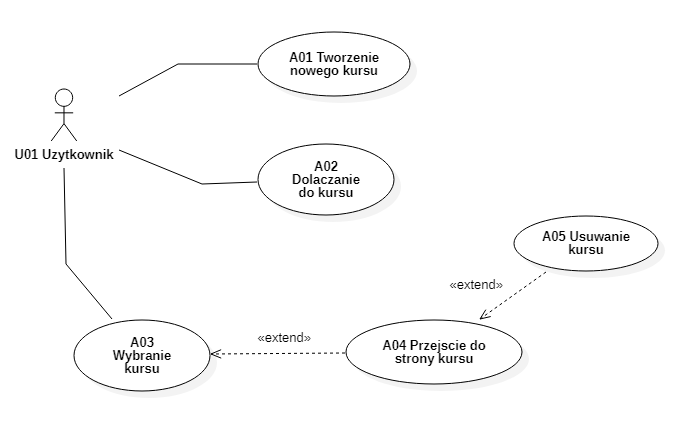
\includegraphics[scale=0.62]{img/chapter4/zarzadzanie_kurs.png}
	\caption{Diagram przypadków użycia, pakiet zarządzanie kursami}
	\label{chapter4_zarzadzanie_kurs}
\end{figure}

\begin{longtable}{|p{1cm}|p{2cm}|p{11cm}|}
    
\caption{Opis przypadków użycia (Zarządzanie kursami)}\\ \toprule
\label{chapter4_tab_usecaseA}
\textbf{ID} &\textbf{Nazwa} & \textbf{Dokumentacja}\\
\midrule


%%%%%%%%%%%%%%%%%%%%%%%%%%%%%%%%%%%%%%%%%% 
A01 & Tworzenie nowego kursu & \vspace{-\baselineskip}
\begin{itemize}[label={-},noitemsep,leftmargin=*,topsep=0pt,partopsep=0pt]
	\item Aktor: Użytkownik
	\item Inicjacja: Wybranie przycisku "dodaj nowy kurs"
	\item Przebieg:
	\begin{enumerate}
		\item system wyświetla formularz do wypełnienia (nazwa, opis, widoczność)
		\item użytkownik wypełnia wszystkie pola w formularzu
		\item użytkownik wybiera przycisk "utwórz kurs"
		\item system przekierowuje użytkownika na stronę administrowania kursem
	\end{enumerate}
\end{itemize} \\\hline
%%%%%%%%%%%%%%%%%%%%%%%%%%%%%%%%%%%%%%%%%%
 
%%%%%%%%%%%%%%%%%%%%%%%%%%%%%%%%%%%%%%%%%%
A02 & Dołączanie do kursu & \vspace{-\baselineskip}
\begin{itemize}[label={-},noitemsep,leftmargin=*,topsep=0pt,partopsep=0pt]
\item Aktor: Użytkownik
\item Inicjacja: Wybranie przycisku "szukaj nowych kursów"
\item Przebieg:
	\begin{enumerate}
		\item system wyświetla listę publicznych kursów
		\item użytkownik wybiera kurs na który chce się zapisać
		\item system wyświetla pytanie z potwierdzeniem 
		\item użytkownik potwierdza chęć dołączenia do kursu
		\item system przekierowuje użytkownika na stronę kursu
	\end{enumerate}
\item Alternatywny przebieg (kurs prywatny)
	\begin{enumerate}
		\item użytkownik wpisuje hasło w polu "dołącz poprzez hasło"
		\item system wyświetla informacje o kursie i pytanie z potwierdzeniem 
		\item użytkownik potwierdza chęć dołączenia do kursu
		\item system przekierowuje użytkownika na stronę kursu
	\end{enumerate}
\end{itemize} \\\hline
%%%%%%%%%%%%%%%%%%%%%%%%%%%%%%%%%%%%%%%%%%
    
%%%%%%%%%%%%%%%%%%%%%%%%%%%%%%%%%%%%%%%%%%
A03 & Wybranie kursu & \vspace{-\baselineskip}
\begin{itemize}[label={-},noitemsep,leftmargin=*,topsep=0pt,partopsep=0pt]
\item Aktor: Użytkownik
\item Inicjacja: Wybranie kursorem danego kursu
\item Przebieg:
	\begin{enumerate}
		\item system wyświetla opis kursu, status (autor/uczestnik), przycisk usuwania oraz przycisk przejścia na stronę kursu
	\end{enumerate}
\end{itemize} \\ \hline
%%%%%%%%%%%%%%%%%%%%%%%%%%%%%%%%%%%%%%%%%%

%%%%%%%%%%%%%%%%%%%%%%%%%%%%%%%%%%%%%%%%%%
A04 & Przejście do strony kursu & \vspace{-\baselineskip}
\begin{itemize}[label={-},noitemsep,leftmargin=*,topsep=0pt,partopsep=0pt]
\item Aktor: Użytkownik
\item Inicjacja: Wybranie przycisku "przejdź na stronę kursu"
\item Przebieg:
	\begin{enumerate}
		\item system przekierowuje użytkownika na odpowiednią stronę kursu w zależności od tego, czy użytkownik jest autorem, czy uczestnikiem
	\end{enumerate}
\end{itemize} \\ \hline
%%%%%%%%%%%%%%%%%%%%%%%%%%%%%%%%%%%%%%%%%%

%%%%%%%%%%%%%%%%%%%%%%%%%%%%%%%%%%%%%%%%%%
A05 & Usuwanie kursu & \vspace{-\baselineskip}
\begin{itemize}[label={-},noitemsep,leftmargin=*,topsep=0pt,partopsep=0pt]
\item Aktor: Użytkownik
\item Inicjacja: Wybranie przycisku "usuń kurs"
\item Przebieg:
	\begin{enumerate}
		\item system wyświetla okno z pytaniem o potwierdzenie usunięcia kursu
		\item użytkownik potwierdza decyzję 
		\item system wyświetla okno z prośbą o wpisanie hasła, by usunąć kurs
		\item użytkownik wpisuje hasło i zatwierdza
		\item system usuwa kurs z listy widocznych kursów
	\end{enumerate}
\item Przebieg alternatywny: (użytkownik nie jest autorem)
	\begin{enumerate}
		\item system wyświetla pytanie o potwierdzenie opuszczenia kursu
		\item użytkownik potwierdza decyzję
		\item system usuwa kurs z listy widocznych kursów 
	\end{enumerate}
\end{itemize} \\\hline
%%%%%%%%%%%%%%%%%%%%%%%%%%%%%%%%%%%%%%%%%%
\end{longtable}